% by pts@fazekas.hu at Fri Aug 28 09:29:30 CEST 2009
%
% Imp: more visual effects (cliparts etc.)
% Imp: no colors in the document size chart
% Imp: add file sizes to the bottom of graph 2
%
% SUXX: pdflatex cannot embed (missing glyph) a Keynote chart with an ff
%       ligature in the caption. Solution: ZERO-WIDH-JOINER unicode char.
\documentclass{beamer}
\usepackage{beamerthemesplit}
\usepackage{lmodern}
\usepackage{t1enc}
\usepackage{graphicx}
\usepackage{ulem}
\usepackage{mflogo}


\definecolor{GoogleBlue}{RGB}{0,102,204}
\definecolor{GoogleRed}{RGB}{255,0,0}
\definecolor{GoogleYellow}{RGB}{255,204,0}
\definecolor{GoogleGreen}{RGB}{0,153,0}
\RequirePackage{xspace}
\newcommand\Google{% The Googley \Google :)
\texorpdfstring{% Color changes do not like to be in bookmarks.
{\color{GoogleBlue}G}%    G
{\color{GoogleRed}o}%     o
{\color{GoogleYellow}o}%  o    :)
{\color{GoogleBlue}g}%    g
{\color{GoogleGreen}l}%   l
{\color{GoogleRed}e}%     e
}{Google}% Colorless text used instead when colors won't work.
\xspace}

\definecolor{c-purple}{rgb}{0.4353,0.2392,0.4745}
\definecolor{c-red}{rgb}{0.7373,0.1765,0.1882}
\definecolor{c-yellow}{rgb}{0.9059,0.6314,0.2392}
\definecolor{c-green}{rgb}{0.3647,0.5882,0.2824}
\definecolor{c-blue}{rgb}{0.1804,0.3412,0.5490}

\title{Optimizing PDF output size of \TeX{} documents}
\subtitle{\ldots{} and PDF files created by other means as well}
\author[P\'eter Szab\'o]{P\'eter Szab\'o\texorpdfstring{\\}{ -- }\textbf{\Google}}
\date{2009-08-31\par\medskip EuroTeX\,2009\\ The Hague, The Netherlands}

%** Create a colorful full square with the specified color.
\def\colorsquare#1{{\color{#1}\vrule width.8em height.8em depth0pt}}

%** Put content to a frame with raggedbottom vertical alignment.
%** This has a hard-coded height for the useful content, depends on the
%** number of sections as well.
%** @example
%**   \frame{
%**      \nocenterframetitle{...}
%**      \nocenter{
%**      ...
%**      }
%**   }
\def\nocenter#1{%
  \hrule height0pt
  \vbox to200pt{\vsize=200pt{\ignorespaces#1}\vfil}%
}

\begin{document}

\frame{\titlepage}

% !!
%\section[Outline]{}
\section{Why and how to optimize?}

\frame{\frametitle{Outline}\tableofcontents}

\subsection{Introduction}

\def\coloremph#1{{\usebeamercolor[fg]{description item}#1}}

\frame{
\frametitle{Why create small PDF files?}
\begin{itemize}
\advance\itemsep1em
\item speed up \coloremph{downloads} (and also reduce download costs)
\item reduce \coloremph{storage} costs
      \begin{itemize}
      \item for publishers, book shops, libraries and print shops
      \item save money everywhere the same PDF is stored
      \end{itemize}
\item use the capacity of \coloremph{e-book readers} more effectively
\end{itemize}
}

\def\conclusionbody{
\begin{itemize}
\advance\itemsep10pt
\item \coloremph{generate quickly,} optimize later
\item \coloremph{no dvips} if possible
\item find the \coloremph{culprit} (fonts, images or drawing instructions)
\item \coloremph{simple techniques} yield the most size reduction
\item optimizing \coloremph{drawing} instructions is hard (and costs money)
\end{itemize}
}

\frame{
\frametitle{To be concluded}
\conclusionbody
}

\frame{
\frametitle{Our PDF optimization approach}
Steps:
\begin{enumerate}
\item \coloremph{generate} the PDF as usual, adjusting only a few, crucial settings
\item \coloremph{repeat} if necessary
\item once the final PDF is ready, \coloremph{optimize} it automatically with one
      or more optimizers
\end{enumerate}
Do not:
\begin{itemize}
\item try to improve or fine-tune \coloremph{every PDF creator software}
\item \coloremph{lose information} (printable or interactive)
      while optimizing
\item use a more compact output
      \coloremph{file format} (such as Multiavalent compact PDF)
\item \coloremph{render} vector graphics
\end{itemize}
}

\frame{
\frametitle{Proposed workflow}
\begin{enumerate}
\advance\itemsep1em
\item follow the best practices for choosing and configuring the
      \coloremph{\TeX{} driver} (pdf\TeX{}, dvipdfm or
      \sout{dvips} + ps2pdf)
\item if affordable, run commercial optimizer \coloremph{PDF Enhancer} or
      \coloremph{Adobe Acrobat} to optimize content streams
\item run our new optimizer called \coloremph{pdfsizeopt.py}
      mainly to optimize images and Type\,1 fonts\par
      \url{http://code.google.com/p/pdfsizeopt/}
\item use \coloremph{Multivalent} \texttt{tool.pdf.Compress} to do the
      rest of the optimization (done automatically by pdfsizeopt.py)
\end{enumerate}
}

\subsection{Optimization techniques}

\frame{
\frametitle{Local techniques are the most effective}
\begin{itemize}
\advance\itemsep1em
\item remove extra \coloremph{whitespace} and comments
\item serialize \coloremph{strings} more effectively
\item compress streams with \coloremph{high-effort ZIP}
     (no RLE, LZW and fax anymore)
\item use \coloremph{cross-reference streams} (with the $y$ predictor)
\item use \coloremph{object streams}
\end{itemize}
}

\frame{
\frametitle{Techniques if data types are known}
\begin{itemize}
\advance\itemsep1em
\item get rid of explicitly specified \coloremph{default} values
\item remove keys \coloremph{ignored} by the PDF specification
\item remove page \coloremph{thumbnails}
\item \coloremph{flatten} the page structure
\item \coloremph{inline} indirect references
      (unless long and there are multiple referrers)
\end{itemize}
}

\frame{
\frametitle{Get rid of duplicate and unused data}
\begin{itemize}
\advance\itemsep1em
\item get rid of \coloremph{unused objects} (pages, images, anchors etc.)
\item compact the \coloremph{cross-reference} tables
\item find \coloremph{duplicate or equivalent} objects, and keep only one copy
\item convert some \coloremph{inline images} to objects to help deduplication
\item \coloremph{split} some large arrays and dictionaries to help
      deduplication
\end{itemize}
}

\frame{
\frametitle{Font optimization techniques}
\begin{itemize}
\advance\itemsep1em
\item convert Type\,1 fonts to \coloremph{CFF} (Type\,1C, Type\,2)
\item \coloremph{subset fonts}
\item \coloremph{unify subsets} of the same font
\end{itemize}
}

\frame{
\frametitle{Image optimization techniques}
\begin{itemize}
\advance\itemsep1em
\item use \coloremph{grayscale or a palette} instead of RGB or CMYK
\item use the smallest \coloremph{bit depth}
\item get rid of image \coloremph{duplicates based on pixel colors}
\item compress with \coloremph{multiple settings}
      (ZIP, ZIP with predictor, JBIG2 or
      combinations) and pick the smallest output
\item compress with \coloremph{high effort} (e.g. slow ZIP with PNGOUT)
\end{itemize}
}

\frame{
\frametitle{Advanced content stream techniques}
If you can calculate on-the-paper bounding boxes, then
\begin{itemize}
\advance\itemsep.25em
\item get rid of \coloremph{objects outside the paper} (and then resubset fonts)
\item get rid of \coloremph{parts of image data} outside the paper
\item do not draw an object if it's \coloremph{covered}
\item \coloremph{clip} vector graphics to the paper rectangle
\end{itemize}
\medskip
Others:
\begin{itemize}
\advance\itemsep.25em
\item \coloremph{flatten} form XObjects, and rebuild them if necessary
\item reorganize \coloremph{graphic-state changing} instructions
\item unify small adjacent images to a large image
\item separate an image for better compressibility
\end{itemize}
}

\subsection{For \TeX{} documents}

\frame{
\frametitle{Drivers: dvipdfm(x) $<$ pdf\TeX{} $\ll$ dvips }
\begin{itemize}
\advance\itemsep1em
\item output of dvips is \coloremph{$>$50\% larger} than any of the other
      drivers
\item dvips output optimized is \coloremph{$>$70\% larger}
\item only dvips supports \coloremph{psfrag} and \coloremph{pstricks}
\item design vector graphics with \coloremph{TikZ or \MP{}}
      (with appropriate helpers) for
      vector graphics instead of \coloremph{pstricks}
\end{itemize}
}

\frame{
\frametitle{Manual setup for small PDF from \TeX{}}
\begin{itemize}
\advance\itemsep1em
\item get rid of \coloremph{complex graphics}
\item reduce \coloremph{image resolution} (300\,DPI or 600\,DPI):
      no need for a higher resolution than the printer's for the scaled image
\item choose the \coloremph{JPEG quality}
\item optimize poorly exported images with \coloremph{sam2p}
\item embed \coloremph{vector fonts}
\item \coloremph{subset fonts} (on by default for \TeX{} text)
\end{itemize}
}

\section{Effectiveness measurements}

\subsection{Input PDF files}

\frame{
\frametitle{Input PDF files}
\begin{description}
\item[cff] \textit{CFF reference}; 62 pages; by \emph{FrameMaker $+$
Distiller}
\item[beamer] first beamer.cls example; 75 slide-steps; by pdf\TeX{}
\item[eu2006] proceedings; 126 pages; by pdf\TeX{} $+$ concat
\item[inkscape] \textit{Inkscape manual}; 341 pages; by \emph{CodeMantra}
\item[lme2006] proceedings in Hungarian; 240 pages; by dvips $+$ ps2pdf $+$ concat
\item[pdfref] \textit{PDF\,1.7 reference} 1310 pages; by \emph{FrameMaker $+$ Distiller}
\item[pgf2] \textit{TikZ manual} 560 pages; by pdf\TeX{}
\item[texbook] \textit{The \TeX{}book} 494 pages; by pdf\TeX{}
\item[tuzv] mini novel in Hungarian; 20 pages; by dvipdfm
\end{description}
}

\frame{
\frametitle{Input PDF sizes}
\nocenter{%
%\vbox to 0pt{}%
%\nointerlineskip
\noindent\hfil
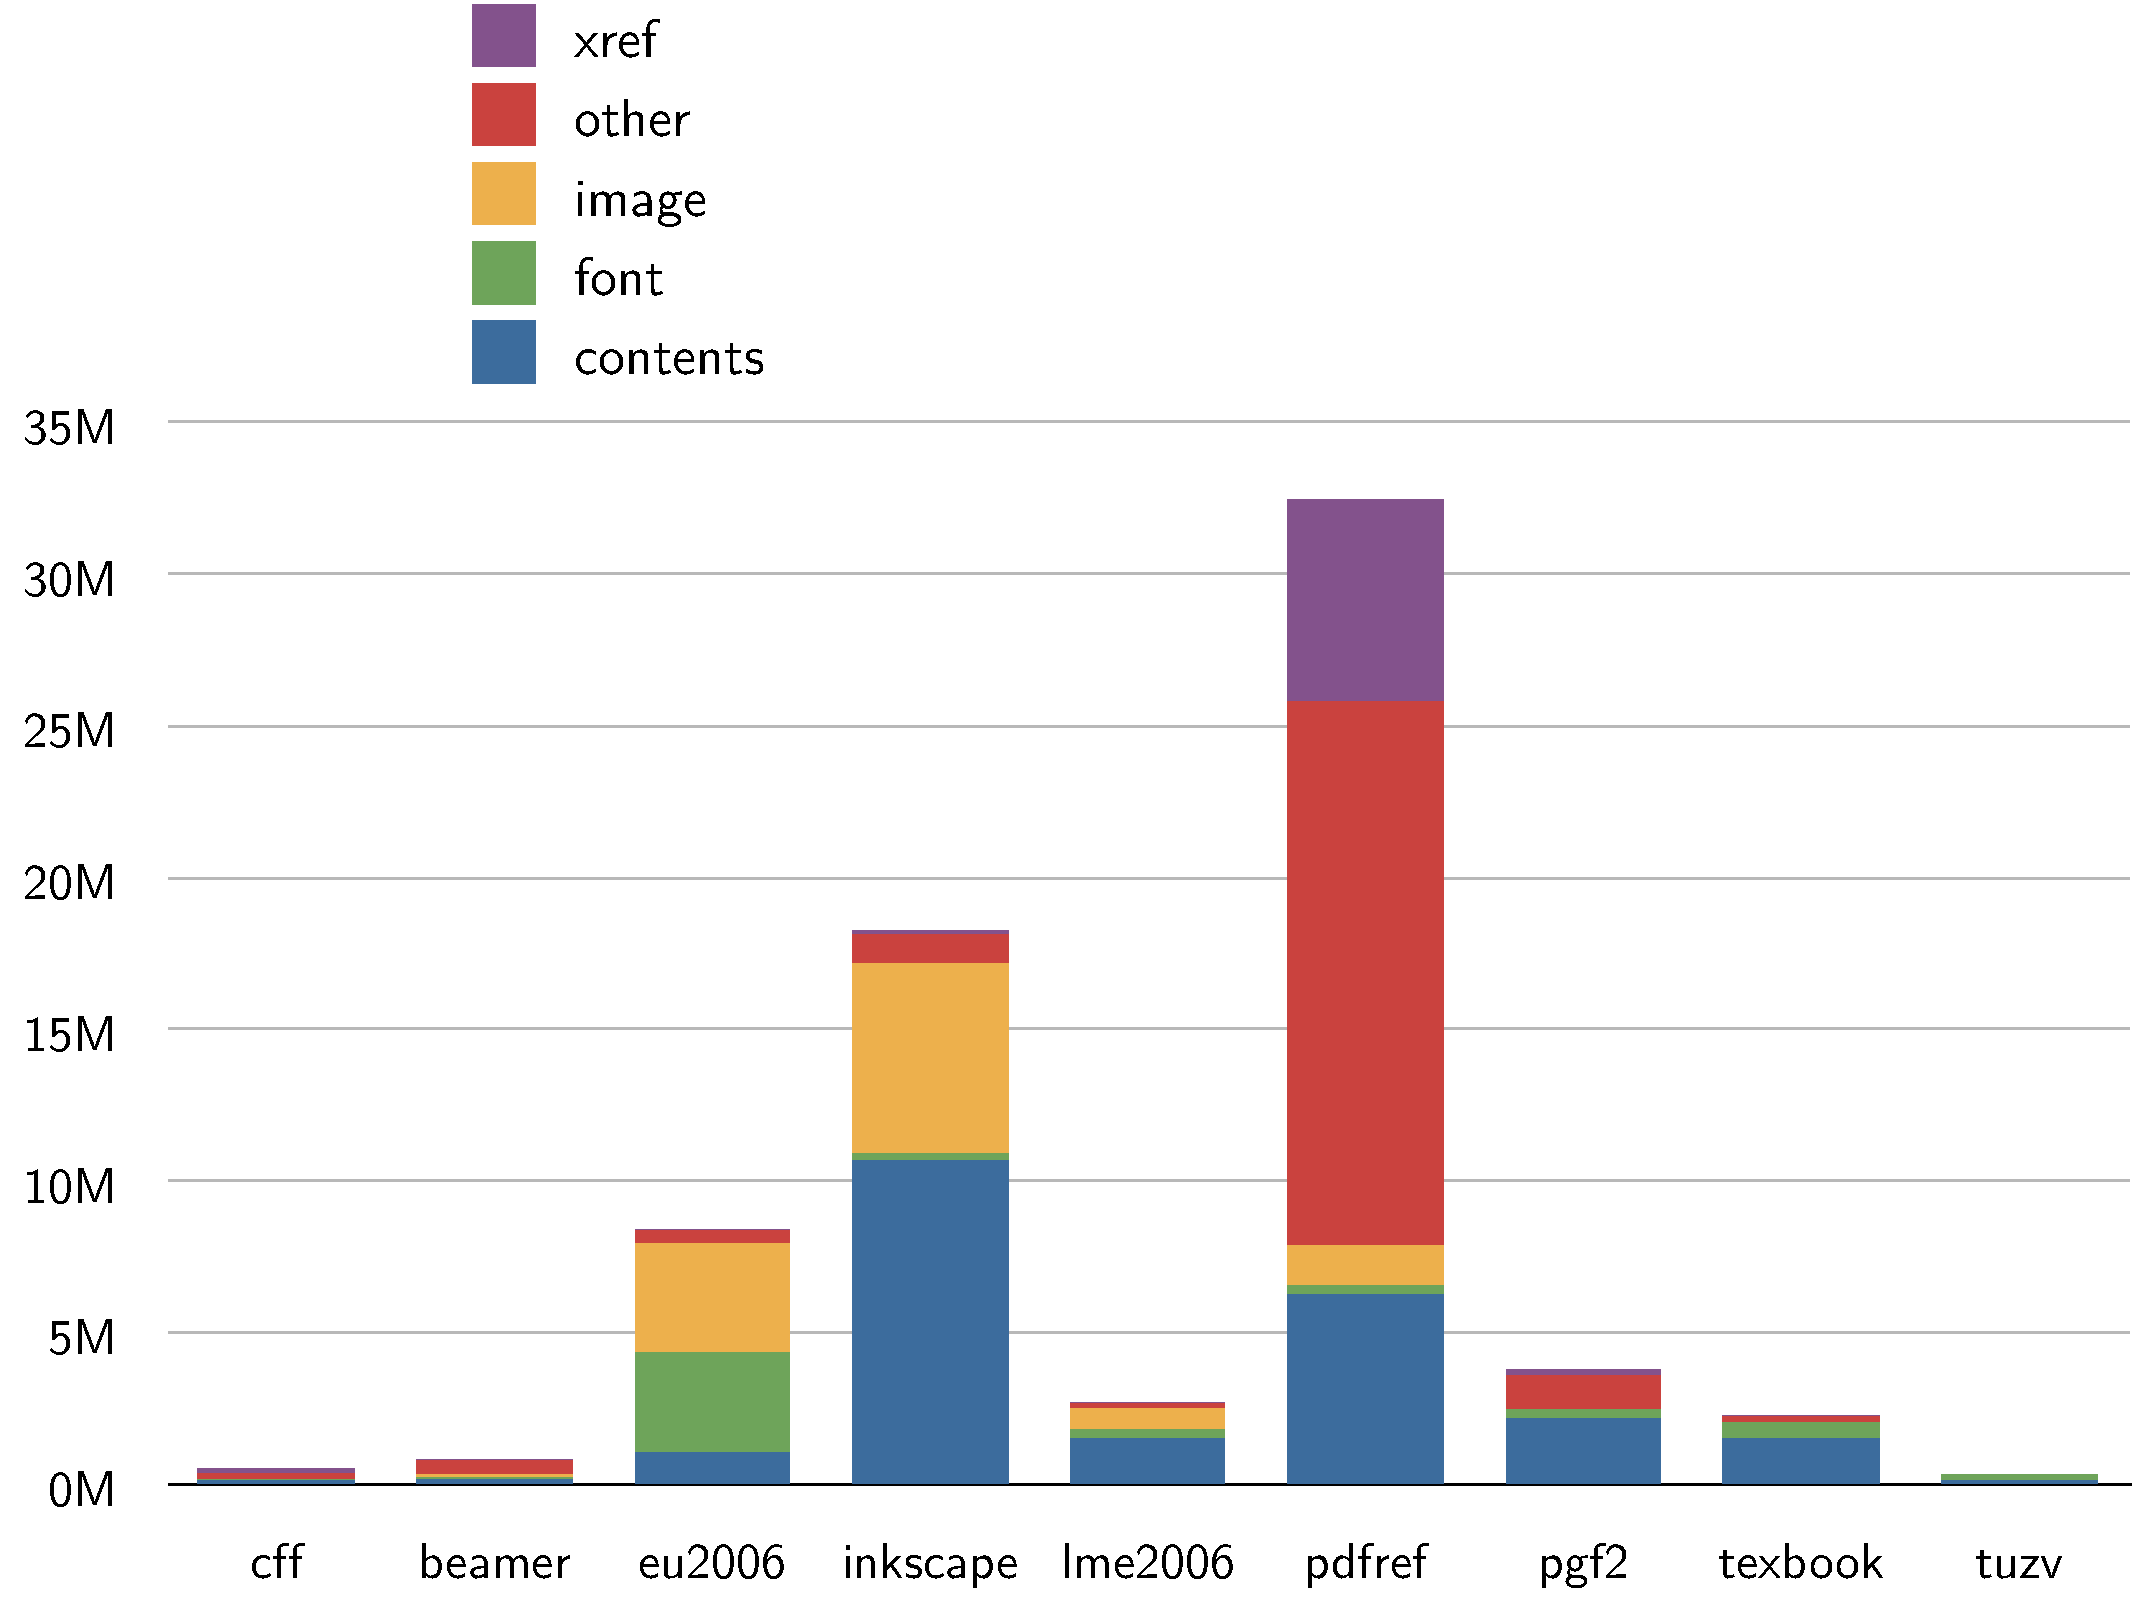
\includegraphics[height=\vsize]{pdfsizeopt_charts_ps2pdf.pdf}
}}

\frame{
\frametitle{PDF features measured}
\begin{description}
\item[xref \colorsquare{c-purple}] cross-reference table containing the document offsets
\item[other \colorsquare{c-red}] hyperlinks, anchors, page structure, section structure
(outlines), submittable forms, and other metadata
\item[image \colorsquare{c-yellow}] embedded pixel images (XObject and inline)
\item[font \colorsquare{c-green}] embedded vector font data
\item[contents \colorsquare{c-blue}] vector graphics, text, colors, patterns
etc., including content streams and form XObjects
\end{description}
}

\frame{
\frametitle{Input PDF feature distribution}
\nocenter{%
\noindent\hfil
\includegraphics[height=\vsize,page=2]{pdfsizeopt_charts_ps2pdf.pdf}
}}

\frame{
\frametitle{Optimizing tools measured}
\begin{itemize}
\advance\itemsep1em
\item input PDF files were optimized using \coloremph{pdfsizeopt.py}
      (calling \coloremph{Multivalent} in its last step)
\item \coloremph{further reductions} are possible (mostly in content
      streams) with Adobe Acrobat and PDF Enhancer (see in the paper)
\item \coloremph{no information was removed} or harmed
\end{itemize}
}

\subsection{Optimization effectiveness charts by feature}

%\frame{
%\frametitle{Image optimization effectiveness (byte sizes)}
%\nocenter{%
%\noindent\hfil
%\includegraphics[height=\vsize,page=3]{pdfsizeopt_charts_ps2pdf.pdf}
%}}

\frame{
\frametitle{Vector graphics and text optimization effectiveness}
\nocenter{%
\noindent\hfil
\includegraphics[height=\vsize,page=4]{pdfsizeopt_charts_ps2pdf.pdf}
}}

\frame{
\frametitle{Embedded font optimization effectiveness}
\nocenter{%
\noindent\hfil
\includegraphics[height=\vsize,page=5]{pdfsizeopt_charts_ps2pdf.pdf}
}}

\frame{
\frametitle{Pixel image optimization effectiveness}
\nocenter{%
\noindent\hfil
\includegraphics[height=\vsize,page=6]{pdfsizeopt_charts_ps2pdf.pdf}
}}

\frame{
\frametitle{Other data optimization effectiveness}
\nocenter{%
\noindent\hfil
\includegraphics[height=\vsize,page=7]{pdfsizeopt_charts_ps2pdf.pdf}
}}

\frame{
\frametitle{Cross-reference optimization effectiveness}
\nocenter{%
\noindent\hfil
\includegraphics[height=\vsize,page=8]{pdfsizeopt_charts_ps2pdf.pdf}
}}

\section{Conclusion}

\frame{
\frametitle{Related work}
\begin{itemize}
\advance\itemsep.5em
\item PDF optimization \coloremph{articles} (mostly lossy)
\item \coloremph{PNG optimizers}
\item other \coloremph{PDF optimizers:} Multivalent, Adobe Acrobat, PDF Enhancer 
\item the \coloremph{PDF Database}
\item \coloremph{DjVu}: at 600\,DPI, 300\% of a text-only PDF; smaller than a PDF for
      images
\item \coloremph{compact PDF} (30\% to 60\% of normal PDF)
\end{itemize}
}

\frame{
\frametitle{Future work}
\begin{itemize}
\advance\itemsep1em
\item get rid of heavy \coloremph{dependencies} (Python, Java, Ghostscript)
      \par $\to$ C++ and Lua from the ground up
\item fix \coloremph{shortcuts}
      \begin{itemize}
      \item support CMYK and other color spaces
      \item better find mergeable CFF fonts
      \item recognize all inline images
      \end{itemize}
\item add \coloremph{test} PDF files (possibly from the PDF database)
\item add \coloremph{concatenetion} support for collections
\end{itemize}
}

\frame{
\frametitle{Conclusion}
\conclusionbody
}

%\subsection{Overview of the Beamer Class}
%\frame
%{
%  \frametitle{Features of the Beamer Class}
%
%  \begin{itemize}
%  \item<1-> Normal LaTeX class.
%  \item<2-> Easy overlays.
%  \item<3-> No external programs needed.      
%  \end{itemize}
%}

\frame{
\thispagestyle{empty}
%\frametitle{hello}
\noindent\hfill{\fontsize{150}{150}\selectfont?}\hfill\null\par
}

\frame{\thispagestyle{empty}}

\end{document}
